%Gồm các nội dung
%1.Tổng quan: Client và server
%2.Đi vào chi tiết các phần ( làm kiểu tương ứng giữa client và server)
% 2.1. Socket
% 2.2. Event: chia làm 3 mục : Màn hình, Chuột, bàn phím
% 2.3. Giao diện

\chapter{Chương trình và mã nguồn}\label{Chapter 2}
\section{Thư viện hỗ trợ}
\section{Tổng quan về mô hình Client - Server}
\subsection{Client}
Trong chương trình của client, ta kết nối với sever thông qua socket để truyền các dữ liệu về màn hình, chuột và bàn phím.
Class \textbf{\ttfamily{Client}} được cài đặt với các thuộc tính và phương thức sau:
    \begin{figure}[H]
	\begin{center}
		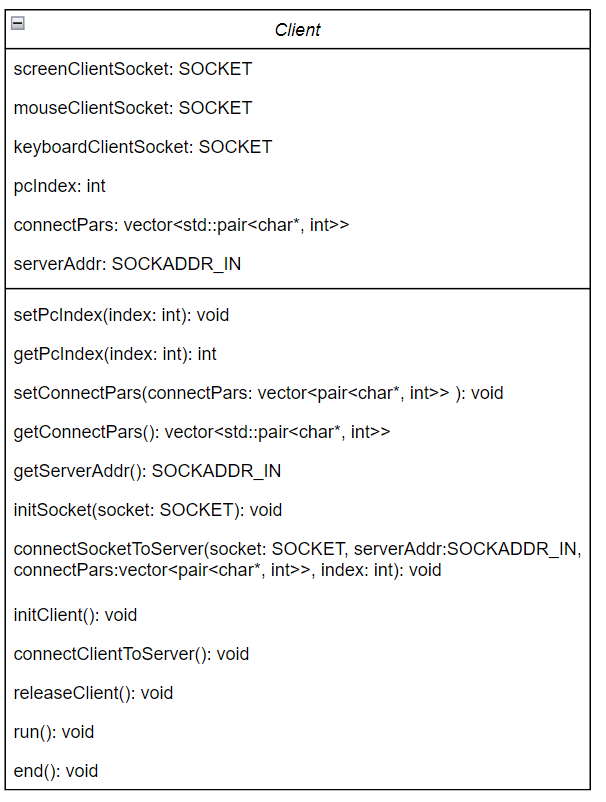
\includegraphics[scale=1.3]{img/client}
            \caption{Sơ đồ class \textbf{\ttfamily{Client}}}
	\end{center}
		
    \end{figure}
\begin{itemize}
        \item Ba socket tương ứng với 3 stream dùng để truyền dữ liệu về màn hình, chuột và bàn phím.
        \item  Các phương thức \textbf{\ttfamily{set, get}} cho các thuộc tính tương ứng được cài đặt như thông thường:
        \item Các phương thức \textbf{\ttfamily{init, connect, release}} thực hiện việc tạo sự liên kết với server phục vụ cho việc truyền nhận dữ liệu. Ta sẽ lần lượt tạo, kết nối và đóng 3 socket ứng với các nhiệm vụ đã trình bày (Cú pháp cụ thể cho một socket sẽ được trình bày tại \ref{clientSocket})
         \begin{figure}[H]
	\begin{center}
		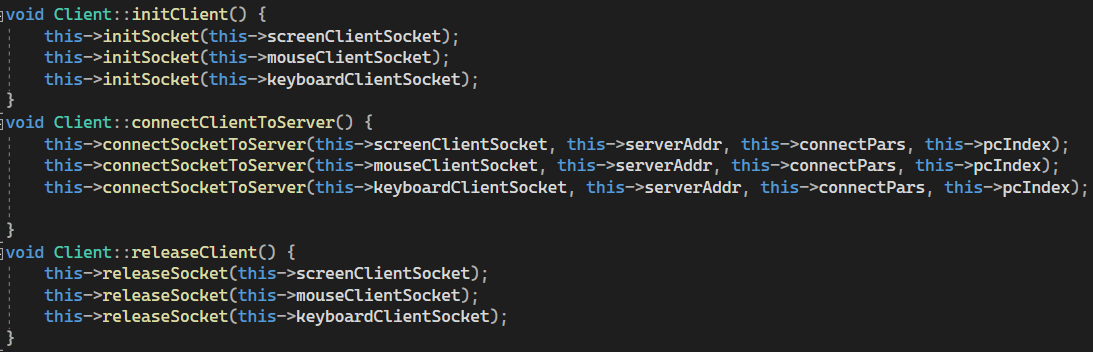
\includegraphics[scale=0.7]{img/clientConnect}
     \caption{Source code: Method \textbf{\ttfamily{init, connect, release.}}}
	\end{center}
		
    \end{figure}
        \item \textbf{\ttfamily{run, end}} thực thi toàn bộ tiến trình truyền và nhận dữ liệu giữa client và server. Trong hàm \textbf{\ttfamily{run}}, tạo ra 3 biến ứng với màn hình, chuột, và bàn phím, sau đó lần lượt gọi phương thức thread của chúng để chạy 3 luồng truyền nhận độc lập (hoạt động của từng luồng sẽ được trình bày rõ tại \ref{events}). Trong hàm \textbf{\ttfamily{end}}, ta lần lượt đóng các stream truyền dữ liệu.
         \begin{figure}[H]
	\begin{center}
		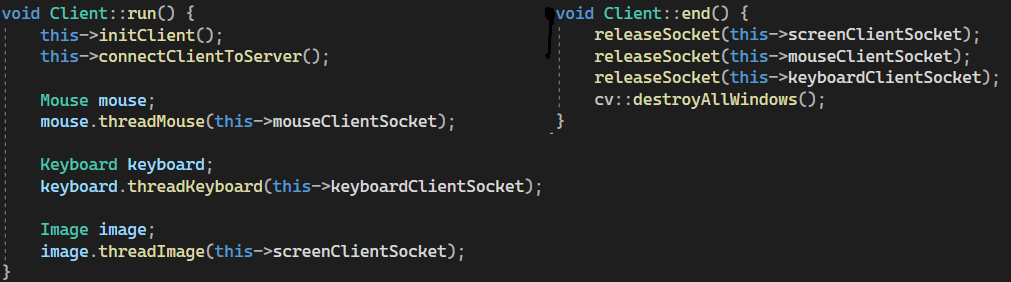
\includegraphics[scale=0.75]{img/clientRunEnd}
    \caption{Source code: Method \textbf{\ttfamily{Run, end}}}
	\end{center}
		
    \end{figure}
\end{itemize}







    
\subsection{Server}














\section{Chi tiết mã nguồn}
\subsection{Socket} \label{socket}
\subsubsection{Client} \label{clientSocket}
\begin{itemize}
    \item \textit{Khởi tạo Socket:} 
    \begin{itemize}
        \item Khai báo một biến có kiểu WSADATA để bắt đầu sử dụng \textbf{Winsock} và kiểm tra đã khởi tạo thành công hay chưa.
        \item Khởi tạo một socket sử dụng địa chỉ IPv4 ($AF\_INET$), và kiểu SOCK$\_$STREAM dùng cho TCP. Kiểm tra việc khởi tại socket.
    \end{itemize}
    \begin{figure}[H]
	\begin{center}
		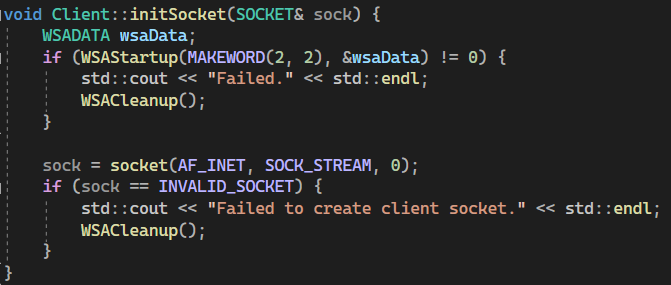
\includegraphics[scale=1]{img/initSocket}
        \caption{Source code: Method \textbf{\ttfamily{initSocket}}}
	\end{center}
		
    \end{figure}
    
    \item \textit{Kết nối Client đến Server thông qua Socket:}
    \begin{itemize}
        \item Lấy địa chỉ ip và port, và thiết lập cấu trúc địa chỉ server (\textbf{\ttfamily{SOCKADRR\_IN}}).
        \item  Kết nối với server thông qua hàm \textbf{\ttfamily{connect}} và kiểm tra có kết nối được hay chưa.
    \end{itemize}
        \begin{figure}[H]
	\begin{center}
		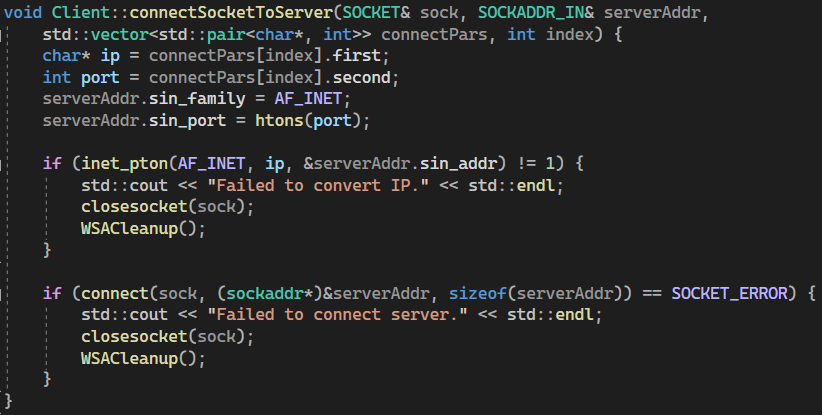
\includegraphics[scale=1]{img/connectSocket.png}
  \caption{Source code: Method \textbf{\ttfamily{connectSocketToServer}}}
	\end{center}	
    \end{figure}
    \item \textit{Đóng Socket:}
        \begin{figure}[H]
	\begin{center}
		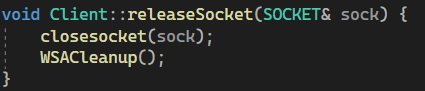
\includegraphics[scale=1.5]{img/releaseSocket}
            \caption{Source code: Method \textbf{\ttfamily{realeaseSocket}}}
	\end{center}
		
    \end{figure}
\end{itemize}





\subsection{Sự kiện} \label{events}
\subsubsection{Màn hình}
\subsubsection{Chuột}
	\textbf{Ý tưởng:}
	\begin{itemize}
		\item \textbf{\textit{Server:}} Sử dụng đồng thời hai luồng (thread) chạy đồng thời để thực hiện nhiệm vụ:
		\begin{itemize}
			\item \textbf{\ttfamily{ReceiveMouseEvent}}: Tiếp nhận thông tin sự kiện chuột (Tọa độ, và sự kiện nhấn, thả hoặc cuộn) và lưu vào biến.  \textbf{\ttfamily{mouseState}}.
			\item \textbf{\ttfamily{putMouse}}: Lấy giá trị của \textbf{\ttfamily{mouseState}} và gửi đến hệ thống.
		\end{itemize}
		\item \textbf{\textit{Client:}}: Sử dụng đồng thời hai luồng (thread) chạy đồng thời để thực hiện nhiệm vụ:
			\begin{itemize}
			\item \textbf{\ttfamily{mouseEventControl}}: Bắt sự kiện chuột (Chỉ lấy các sự kiện được diễn ra trong phạm vi window hiển thị màn hình của server) và lưu vào biến.  \textbf{\ttfamily{mouseState}}.
			\item \textbf{\ttfamily{sendMouseInfomation}}: Lấy giá trị của \textbf{\ttfamily{mouseState}} và gửi đến server.
		\end{itemize}
	\end{itemize}
\textbf{Cài đặt hàm:}
	\begin{itemize}
		\item Định nghĩa một enum  class \textbf{\ttfamily{MouseEvent}} để định nghĩa các sự kiện chuột (tránh xung đột tên):
			\begin{figure}[H]
			\begin{center}
				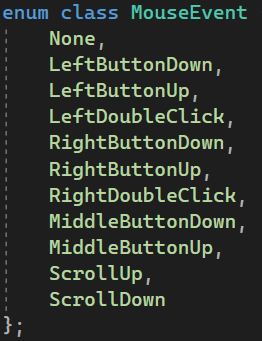
\includegraphics[scale=1]{img/enumClassMouse}
                 \caption{Souce code: Enum class \textbf{\ttfamily{MouseEvent}}}
			\end{center}
		\end{figure}
		\item Định nghĩa class \textbf{\ttfamily{Mouse}} với các thuộc tính \textbf{\ttfamily{coordinate, event}} tương ứng với tọa độ và sự kiện (nhấn, thả, cuộn) chuột và cài đặt các phương thức  \textbf{\ttfamily{constructor, set, get}} tương ứng:
			\begin{figure}[H]
			\begin{center}
				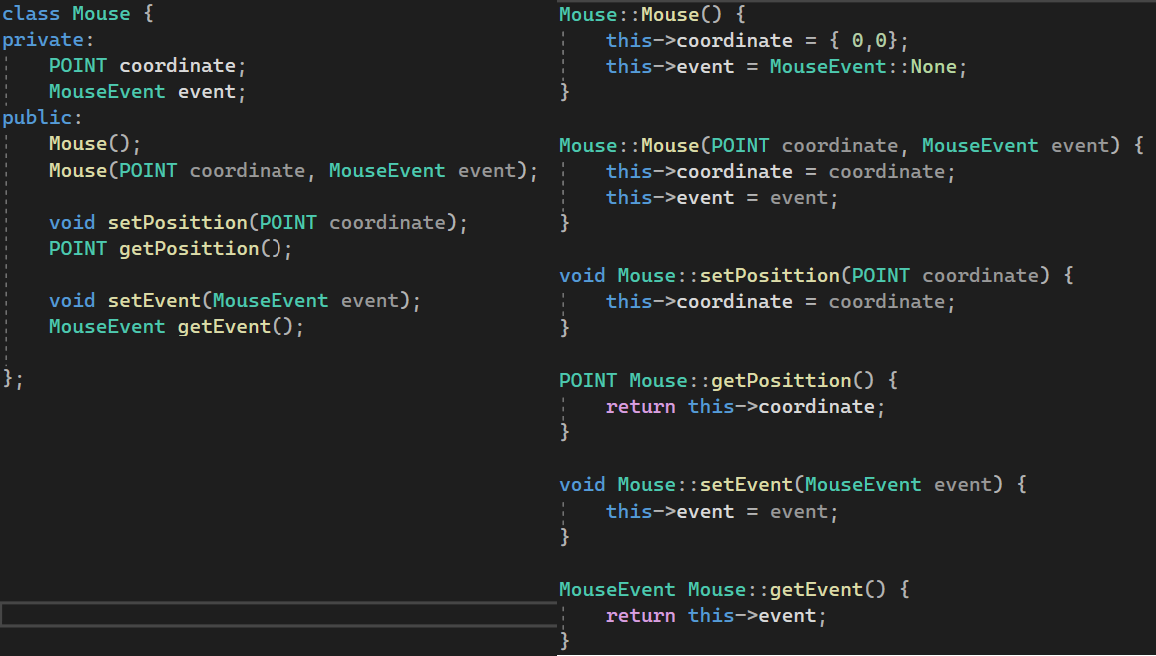
\includegraphics[scale=0.63]{img/mouseClass}
                  \caption{Souce code: Class \textbf{\ttfamily{Mouse}}}   
			\end{center}
		\end{figure}
	
		\item \textbf{\textit{Server:}}
		\begin{itemize}
			\item \textbf{\ttfamily{void ReceiveMouseEvent(SOCKET clientSocket)}}\\
			 \textit{Tiếp nhận thông tin sự kiện chuột: }
			 \begin{itemize}
			 	\item  Sử dụng một buffer để lưu dữ liệu nhận được từ client thông qua \textbf{\ttfamily{clientSocket}}.
			 	\item Nhận dữ liệu và kiểm tra có nhận được dữ liệu thành công hay không.
			 \end{itemize}
			 \textit{Lưu thông tin sự kiện chuột biến} \textbf{\ttfamily{mouseState}}:
			 \begin{itemize}
			 	\item Đọc dữ liệu từ buffer (thông qua hàm \textbf{\ttfamily{memcopy)}}).
			 	\item Chuyển đổi dữ liệu nhận được thành các giá trị tọa độ, sự kiện chuột có kiểu dữ liệu tương ứng với các thuộc tính của biến \textbf{\ttfamily{mouseState}}.
			 	\item Lưu các dữ liệu trên vào biến \textbf{\ttfamily{mouseState}} thông qua các phương thức \textbf{\ttfamily{setPosittion, setEvent}}.
			 \end{itemize}
				\begin{figure}[H]
				\begin{center}
					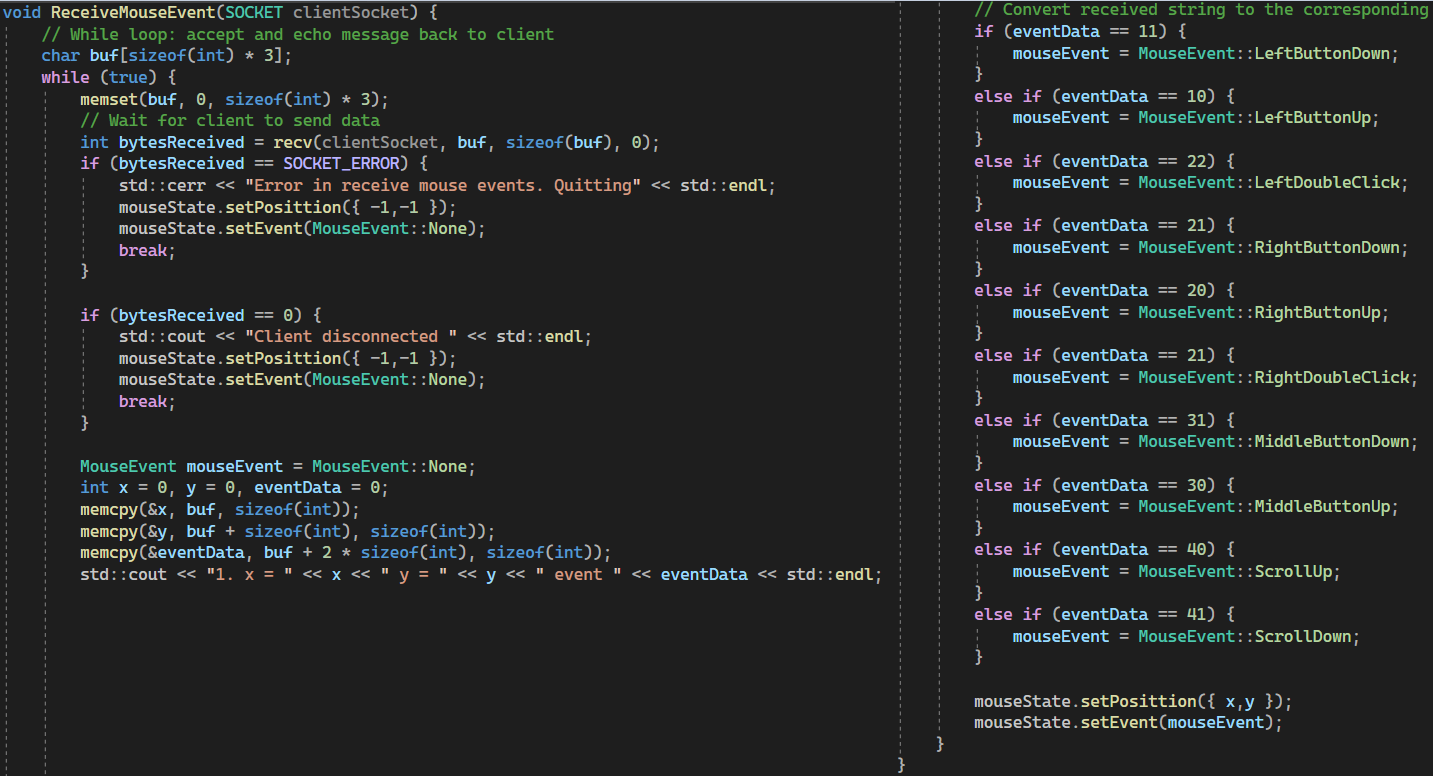
\includegraphics[scale=0.56]{img/recvMouse}
                        \caption{Souce code: Function
				\end{center}
					 \textbf{\ttfamily{ReceiveMouseEvent}}}
			\end{figure}
		
		\item \textbf{\ttfamily{void putMouse()}}: Sử dụng 1 vòng lặp (có độ trễ 1ms) để liên tục thực hiện:
		\begin{itemize}
			\item Chuyển đổi thông tin chuột mouseState để set giá trị cho các thuộc tính của biến \textbf{\ttfamily{input}}.
			\item Gửi dữ liệu chuột đến hên hệ thống thông qua hàm \textbf{\ttfamily{SendInput}} và \textbf{\ttfamily{setCursorPos}}
			\begin{figure}[H]
				\begin{center}
					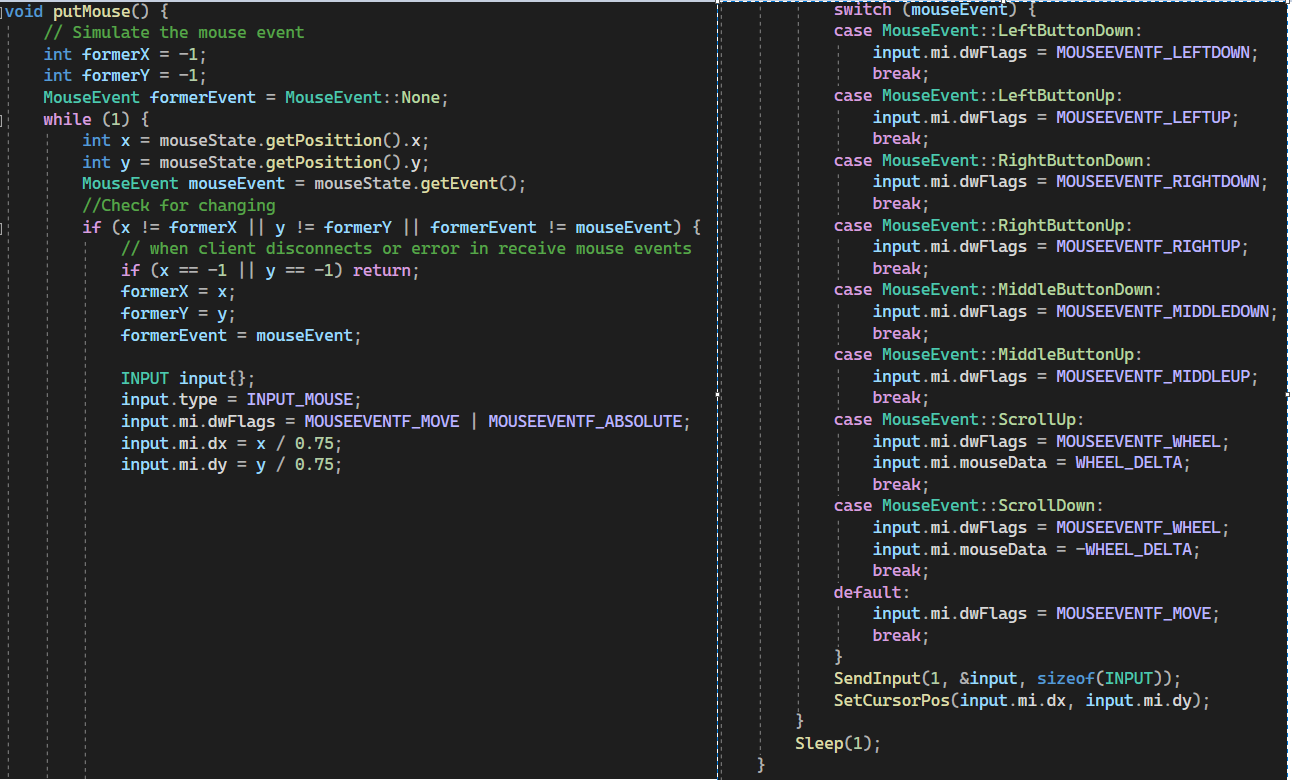
\includegraphics[scale=0.625]{img/putMouse}
                        \caption{Souce code: Function \textbf{\ttfamily{putMouse}}}
				\end{center}
			\end{figure}
		\end{itemize}	
		\end{itemize}
	\item \textbf{\textit{Client:}}\\
	\textit{Tiến trình lấy sự kiện chuột:}
	\begin{itemize}
		\item \textbf{\ttfamily{cv::setMouseCallback("Virtual Machine Screen", mouseEventControl, NULL)}}\\
		Hàm callback để liên tục bắt sự kiện chuột khi có sự kiện chuột xảy ra trong window hiển thị màn hình server. Hàm này chạy chung luồng với tiến trình hiện ảnh của màn hình server.
		\item  \textbf{\ttfamily{void mouseEventControl(int event, int x, int y, int flags, void* userData)}} \\
		Sử dụng thông tin nhận được từ hàm callback ở trên để set giá trị cho các thuộc tính của biến \textbf{\ttfamily{mouseState}}.
		\begin{figure}[H]
			\begin{center}
				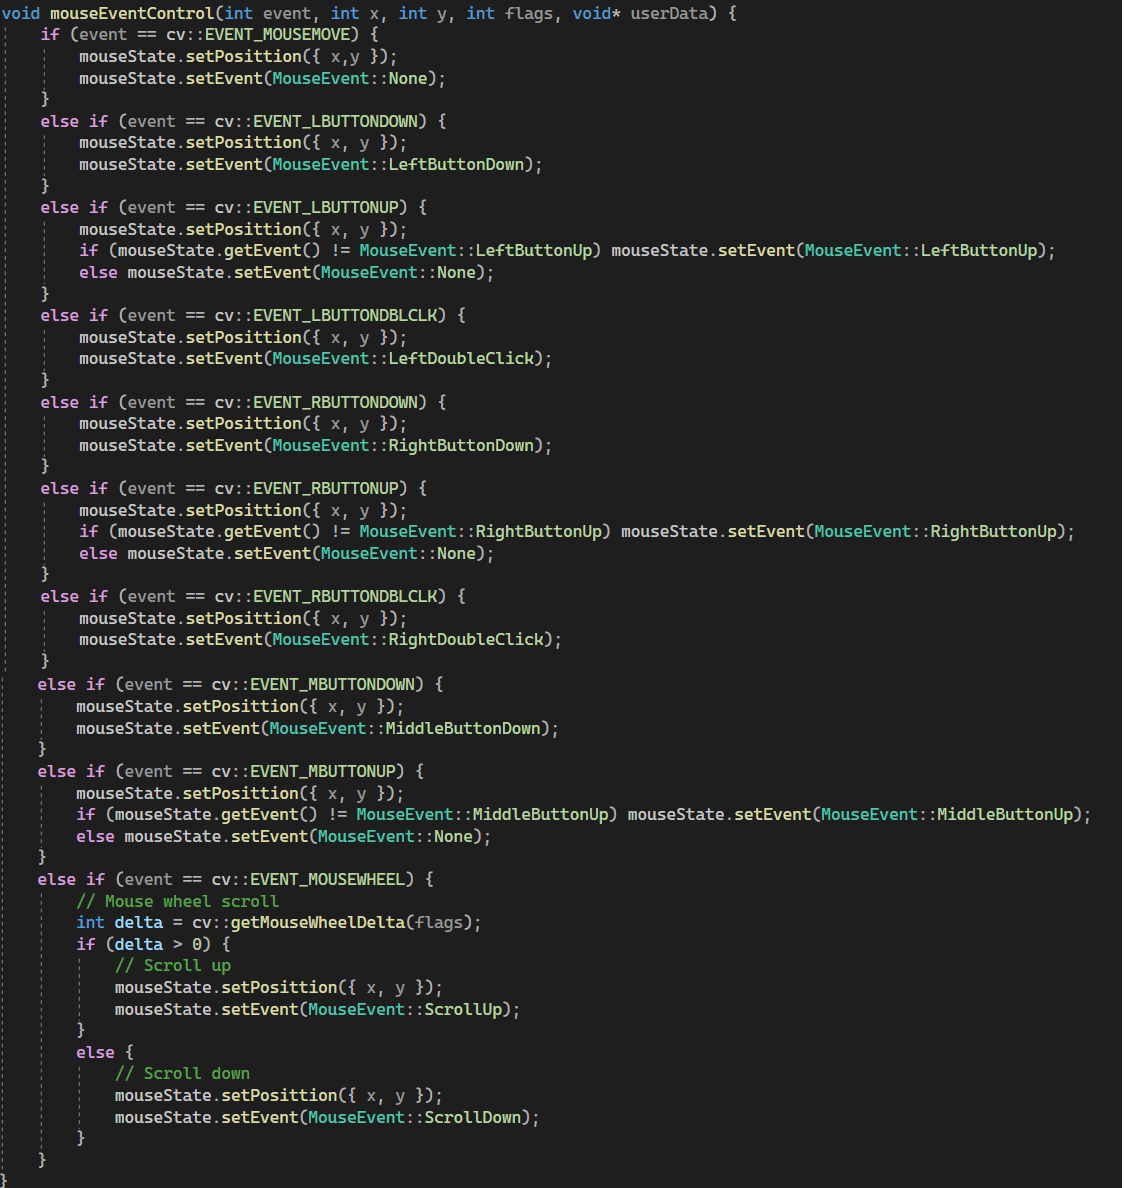
\includegraphics[scale=0.7]{img/mouseControl}
            \caption{Souce code: Function\textbf{\ttfamily{mouseEventControl}}}
			\end{center}
			
		\end{figure}
	\end{itemize}
	\textit{Tiến trình gởi sự kiện chuột đến server:}
	\begin{itemize}
		\item \textbf{\ttfamily{bool getBufferMouseInformation(char* buf)}}\\
		Lưu các thông tin về vị trí và sự kiện chuột vào trong một buffer để chuẩn bị cho việc gởi dữ liệu đến server.
			\begin{figure}[H]
			\begin{center}
				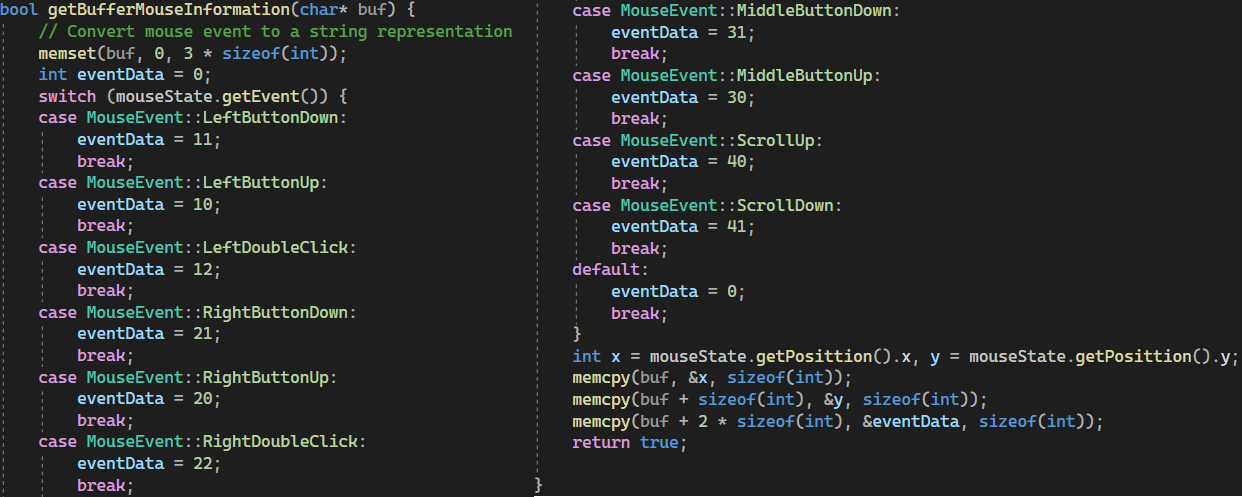
\includegraphics[scale=0.65]{img/getMouseBuf}
                \caption{Souce code: Function \textbf{\ttfamily{getBufferMouseInformation}}}
			\end{center}
			
		\end{figure}
		\item \textbf{\ttfamily{void sendMouseInfomation(SOCKET sock)}}\\
	Kiểm tra tọa độ và sự kiện chuột, nếu có sự thay đổi thì tiến hành tạo buffer, lấy thông tin chuột lưu vào buffer và gởi đến server.
	\begin{figure}[H]
		\begin{center}
			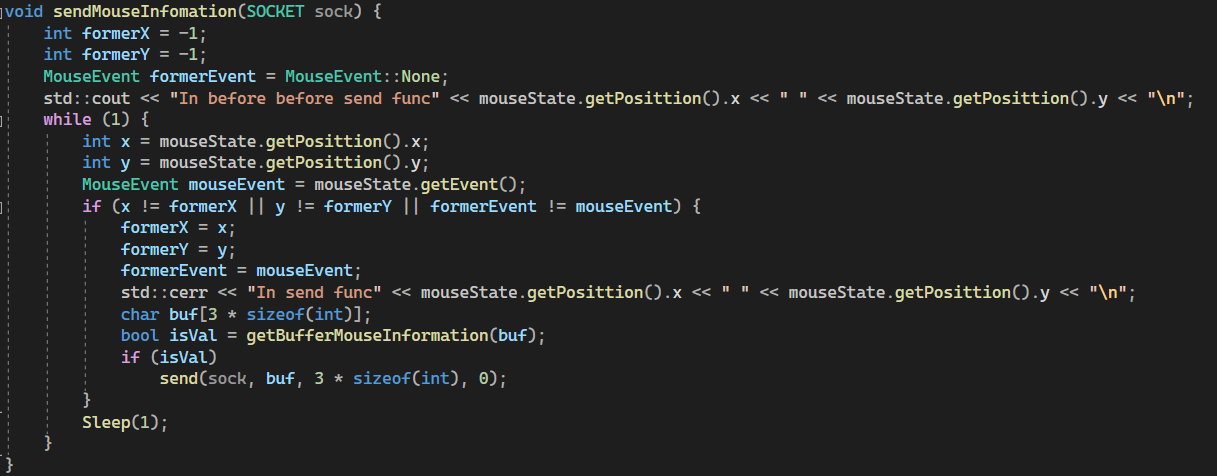
\includegraphics[scale=0.66]{img/sendMouse}
                  \caption{Souce code: Function \textbf{\ttfamily{sendMouseInfomation}}}
		\end{center}
	\end{figure}
	\end{itemize}
	 \textit{Tiến trình gởi thông tin chuột được chạy độc lập trong một luồng riêng biệt.}
		\begin{figure}[H]
		\begin{center}
			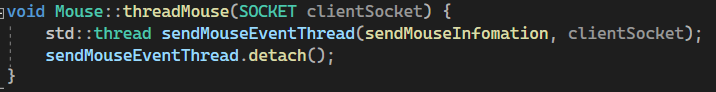
\includegraphics[scale=1]{img/mouseThread}
                \caption{Souce code: \textbf{\ttfamily{threadMouse}}}
		\end{center}
		
	\end{figure}
\end{itemize}










\subsubsection{Bàn phím}
Ở phần này em sẽ giới thiệu về sự kiện của bàn phím trong đồ án của nhóm em.
\begin{itemize}
    \item client \\
    các hàm được sử dụng trong client bao gồm: \\
    \begin{figure}[H]
    \begin{center}
    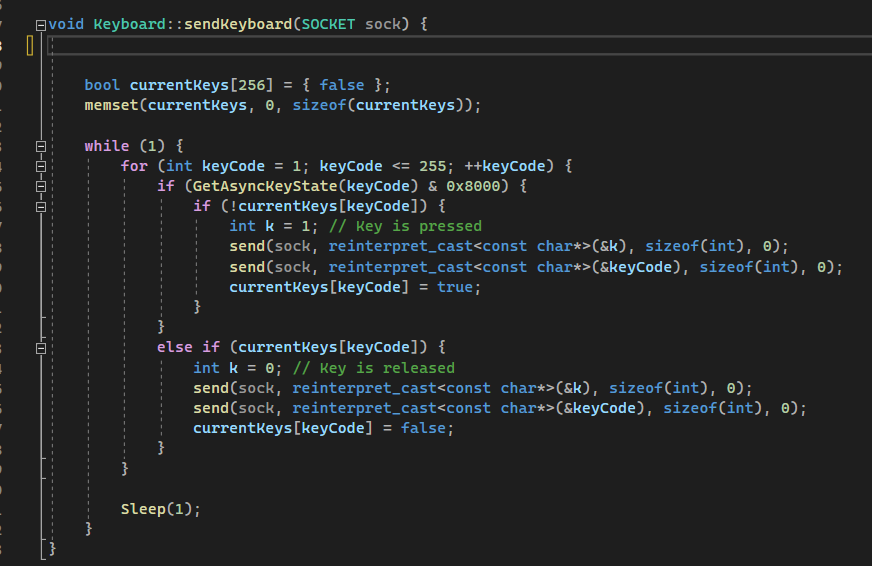
\includegraphics[scale=0.8]{img/sendKeyboard.png}
    \caption{soure code của hàm \textbf{\ttfamily{sendKeyboard}}}
    \end{center}
    \end{figure}
    Hàm \textbf{\ttfamily{sendKeyboard}} có chức năng gửi thông tin về các phím được nhấn và nhả ra từ bàn phím tới một \textbf{\ttfamily{SOCKET}} (socket) đã được thiết lập.\\
    Cụ thể, hàm này có các bước thực hiện sau:
    \begin{itemize}
    \item[$-$] Khởi tạo một mảng  \textbf{\ttfamily{currentKeys}} gồm 256 phần tử, ban đầu tất cả các phần tử đều được đặt giá trị false. Mảng này sẽ lưu trạng thái của các phím, dùng để xác định xem một phím đã được nhấn hay đã được nhả ra.
    \item[$-$] Trong vòng lặp vô hạn (while (1)), hàm sẽ duyệt qua từng mã phím từ 1 tới 255 để kiểm tra xem các phím đó có đang được nhấn hay không.
    \item[$-$] Đối với mỗi mã phím (\textbf{\ttfamily{keyCode}}), hàm sẽ sử dụng hàm \textbf{\ttfamily{GetAsyncKeyState}} để kiểm tra xem phím có đang được nhấn không. Nếu phím đang được nhấn (\textbf{\ttfamily{GetAsyncKeyState(keyCode) \& 0x8000}}), và trạng thái trước đó của phím là không được nhấn (\textbf{\ttfamily{!currentKeys[keyCode]}}), hàm sẽ thực hiện các bước sau:\\
    a. Gửi một số nguyên 1 (\textbf{\ttfamily{int k = 1}}) thông qua socket sock, để chỉ định rằng một phím đã được nhấn.\\
    b. Gửi mã phím (\textbf{\ttfamily{keyCode}}) thông qua socket sock, để truyền thông tin về phím nào đã được nhấn.\\
    c. Đánh dấu phím hiện tại (\textbf{\ttfamily{currentKeys[keyCode]}}) là đã được nhấn (true).\\
    \item[$-$] Trong trường hợp phím không được nhấn (\textbf{\ttfamily{keyCode])}}), tức là phím đã được nhấn trước đó nhưng không còn được nhấn nữa, hàm sẽ thực hiện các bước sau:\\
    a. Gửi một số nguyên 0 (\textbf{\ttfamily{int k = 0}}) thông qua socket sock, để chỉ định rằng một phím đã được nhả ra (không còn được nhấn).\\
    b. Gửi mã phím (\textbf{\ttfamily{keyCode}}) thông qua socket sock, để truyền thông tin về phím nào đã được nhả ra.\\
    c. Đánh dấu phím hiện tại (\textbf{\ttfamily{currentKeys[keyCode]}}) là không được nhấn (false).
    \item[$-$] Cuối cùng, sau khi kiểm tra tất cả các mã phím từ 1 tới 255, hàm sẽ dừng một khoảng thời gian ngắn (\textbf{\ttfamily{Sleep(1)}}) trước khi tiếp tục vòng lặp.
    \end{itemize}
    hàm \textbf{\ttfamily{sendKeyboard}} này sẽ liên tục gửi thông tin về trạng thái của các phím được nhấn và nhả ra từ bàn phím tới một socket đã được thiết lập.\\

    \begin{figure}[H]
    \begin{center}
    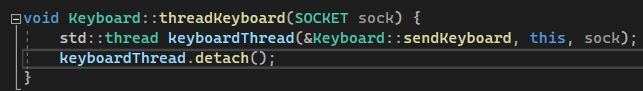
\includegraphics[scale=0.8]{img/threadKeyboard.png}
    \caption{soure code của hàm \textbf{\ttfamily{threadKeyboard}}}
    \end{center}
    \end{figure}
    Hàm \textbf{\ttfamily{threadKeyboard}} có chức năng tạo một luồng (\textbf{\ttfamily{thread}}) mới để thực thi hàm \textbf{\ttfamily{sendKeyboard}} trong lớp \textbf{\ttfamily{Keyboard}}.\\
    Cụ thể, hàm này có các bước thực hiện sau:
    \begin{itemize}
        \item[$-$] Tạo một đối tượng luồng (\textbf{\ttfamily{keyboardThread}}) từ lớp \textbf{\ttfamily{std::thread}}. Hàm \textbf{\ttfamily{std::thread}} nhận vào một con trỏ hàm thành viên và các đối số liên quan để tạo một luồng mới. Trong trường hợp này, con trỏ hàm thành viên được truyền vào là \textbf{\ttfamily{\&Keyboard::sendKeyboard}}, tức là hàm \textbf{\ttfamily{sendKeyboard}} trong lớp \textbf{\ttfamily{Keyboard}}.
        \item[$-$]Đối tượng luồng (\textbf{\ttfamily{keyboardThread}}) được khởi tạo với các đối số sau:\\
        this: Con trỏ đối tượng hiện tại (được sử dụng để truy cập vào thành viên và phương thức của lớp).\\
        sock: Socket được truyền vào từ đối số của hàm \textbf{\ttfamily{threadKeyboard}}.
        \item[$-$]Gọi phương thức \textbf{\ttfamily{detach()}} trên đối tượng luồng (\textbf{\ttfamily{keyboardThread}}). Phương thức \textbf{\ttfamily{detach()}} được sử dụng để tách luồng mới tạo ra từ luồng chính. Điều này có nghĩa là luồng mới sẽ tiếp tục thực thi độc lập và không cần phụ thuộc vào luồng chính. Trong trường hợp này, luồng \textbf{\ttfamily{keyboardThread}} sẽ thực thi hàm \textbf{\ttfamily{sendKeyboard}} trong lớp \textbf{\ttfamily{Keyboard}} mà không cần sự can thiệp của luồng gọi \textbf{\ttfamily{threadKeyboard}}.
    \end{itemize}
    hàm \textbf{\ttfamily{threadKeyboard}} tạo một luồng mới và thực thi hàm \textbf{\ttfamily{sendKeyboard}} trong lớp \textbf{\ttfamily{Keyboard}} trên luồng đó. Sau đó, luồng mới được tách ra và tiếp tục thực thi độc lập với luồng gọi \lstinline[language=C++]|threadKeyboard|. Điều này cho phép việc gửi thông tin từ bàn phím thông qua socket (sock) được thực hiện trong một luồng riêng biệt mà không làm chặn luồng chính.
    \item  server \\
    các hàm được sử dụng trong server bao gồm:\\
    \begin{figure}[H]
    \begin{center}
    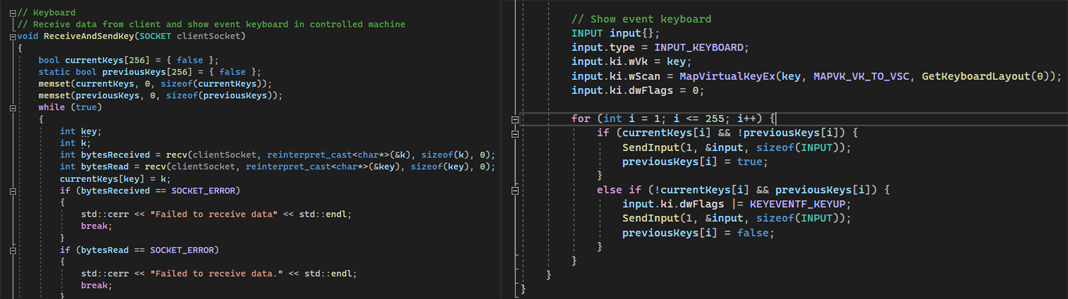
\includegraphics[scale=0.5]{img/ReceiveAndSendKey.png}
    \caption{soure code của hàm \textbf{\ttfamily{ReceiveAndSendKey}}}
    \end{center}
    \end{figure}
    \begin{itemize}
        \item[$-$] Mảng \textbf{\ttfamily{currentKeys}} và \textbf{\ttfamily{previousKeys}} được khởi tạo với giá trị mặc định là false cho tất cả các phần tử. Mảng \textbf{\ttfamily{currentKeys}} lưu trữ trạng thái hiện tại của các phím, trong khi mảng \textbf{\ttfamily{previousKeys}} lưu trữ trạng thái trước đó của các phím.
        \item[$-$] Hai lệnh \textbf{\ttfamily{memset}} được sử dụng để đặt tất cả các phần tử của \textbf{\ttfamily{currentKeys}} và \textbf{\ttfamily{previousKeys}} về 0. Điều này đảm bảo rằng các mảng có giá trị ban đầu là false.
        \item[$-$] Một vòng lặp vô hạn (\textbf{\ttfamily{while (true)}}) được sử dụng để liên tục nhận và xử lý thông tin từ client.
        \item[$-$] Hai lệnh \textbf{\ttfamily{recv}} được sử dụng để nhận dữ liệu từ socket. Đầu tiên, recv nhận thông tin về trạng thái của phím (k), sau đó \textbf{\ttfamily{recv}} nhận giá trị mã của phím (\textbf{\ttfamily{key}}). Dữ liệu được nhận được gán cho \textbf{\ttfamily{currentKeys[key]}} để cập nhật trạng thái hiện tại của phím.
        \item[$-$] Hai câu điều kiện \textbf{\ttfamily{i}} được sử dụng để kiểm tra xem việc nhận dữ liệu có thành công hay không. Nếu có lỗi xảy ra trong quá trình nhận dữ liệu, thông báo lỗi sẽ được in ra màn hình và vòng lặp sẽ được thoát.
        \item[$-$] Một đối tượng \textbf{\ttfamily{INPUT}} mới được khởi tạo, đại diện cho một sự kiện bàn phím. Các thuộc tính của đối tượng \textbf{\ttfamily{INPUT}} được thiết lập để phù hợp với phím được nhận. \textbf{\ttfamily{input.type}} được đặt thành \textbf{\ttfamily{INPUT\_KEYBOARD}} để chỉ định rằng đây là một sự kiện bàn phím. \textbf{\ttfamily{input.ki.wVk}} được gán bằng giá trị mã phím, \textbf{\ttfamily{input.ki.wScan}} được gán bằng mã quét của phím, và \textbf{\ttfamily{input.ki.dwFlags}} được đặt thành 0 ban đầu.
        \item[$-$] Một vòng lặp từ i = 1 đến 255 được sử dụng để duyệt qua tất cả các phím. Trong vòng lặp này, các câu điều kiện \textbf{\ttfamily{i}}f kiểm tra trạng thái của từng phím.
        \item[$-$] Nếu \textbf{\ttfamily{currentKeys[i]}} là true và \textbf{\ttfamily{previousKeys[i]}} là \textbf{\ttfamily{false}}, tức là phím i đã được nhấn và trước đó không được nhấn, sự kiện bàn phím nhấn sẽ được gửi tới hệ thống bằng hàm \textbf{\ttfamily{SendInput}}. Sau đó, \textbf{\ttfamily{previousKeys[i]}} được cập nhật thành true.
        \item[$-$] Ngược lại, nếu \textbf{\ttfamily{currentKeys[i]}} là \textbf{\ttfamily{false}} và \textbf{\ttfamily{previousKeys[i]}} là \textbf{\ttfamily{true}}, tức là phím i đã được nhả ra sau khi được nhấn trước đó, sự kiện bàn phím nhả ra sẽ được gửi tới hệ thống bằng cách thiết lập cờ \textbf{\ttfamily{KEYEVENTF\_KEYUP}} trong \textbf{\ttfamily{input.ki.dwFlags}} và gửi thông tin sự kiện phím bằng hàm \textbf{\ttfamily{SendInput}}. Sau đó, \textbf{\ttfamily{previousKeys[i]}} được cập nhật thành \textbf{\ttfamily{false}}.
    \end{itemize}
\end{itemize}
\subsection{Giao diện}